\section{Experimental Evaluation}
\label{sec:evaluation}

This section aims to answer the following research questions: 

\begin{itemize}
\item \textbf{Performance:} How is \NM{}'s performance, comparing to popular general allocators and NUMA-aware allocators? (Section~\ref{sec:performance}) 
\item \textbf{Memory Consumption:} What is the memory consumption of \NM{}? (Section~\ref{sec:memory})
\item \textbf{Scalability:} How is the scalability of \NM{}? (Section~\ref{sec:scale})
\item \textbf{Impact of Design Choices:} How important every design choice can actually impact performance? (Section~\ref{sec:design})	
\end{itemize}

\begin{comment}

\begin{table}[!ht]
 \centering
   \caption{Machine specifications for evaluation
   \label{table:Machine}}
  %\setlength{\tabcolsep}{1.0em}
\begin{tabular}{l | l }
\hline
Category & Information \\ \hline
CPUs/Model 	& Xeon(R) Platinum 8153\\ \hline
CPU Frequency & 2.00GHz\\ \hline
NUMA Nodes  & 8 \\ \hline
Physical Cores  & 8$\times$16 \\ \hline
Node Latency &  \specialcell{local: 1.0 \\ 1 hop: 2.1 \\ 2 hops: 3.1}\\ \hline
Interconnect Bandwidth  & 10.4GT/s\\ \hline
Linux & Debian 10\\ \hline
Compiler &  GCC-8.3.0 \\ \hline
%Memory Bandwidth & 19.87 GB/s & \\ \hline
  \end{tabular}
  %\vspace{-0.4in}
\end{table}
\end{comment}

\textbf{Experimental Setup:}  \NM{} was evaluated on an Intel Xeon(R) Platinum 8153 machine with 8 nodes, where each node has 16 cores. Any two nodes are less than or equal to 3 hops, where the latency of two hops and three hops is 2.1 and 3.1 separately if the latency of local accesses is 1.0. The machine is installed with 512GB memory. The underlying OS is Linux Debian 10 and the compiler is GCC-8.3.0. For the evaluation, the hyperthreading was turned off, but both transparent page support and AutoNUMA are  enabled. The performance data shown in this paper is the average of 10 runs, in order to avoid any bias caused by unexpected events.  

\textbf{Compared Baseline and Evaluated Applications: }  We compare \NM{} with multiple popular allocators, such as the default Linux allocator, TCMalloc~\cite{tcmalloc2},  TCMalloc-NUMA~\cite{tcmallocnew}, jemalloc-5.2.1~\cite{jemalloc}, Intel TBB-2021.5~\cite{tbb2}, Scalloc-1.0.0~\cite{Scalloc}, and mimalloc~\cite{mimalloc}. Note that we are comparing against the TCMalloc's NUMA awareness version (released on July 2021), and the newest version of TBB (with numa support, released on December 2021). 
%Among them, TCMalloc, jemalloc, TBB, and mimalloc are commercial allocators designed and maintained by Industrial Giants, like Google, Facebook, Intel, and Microsoft separately. 
We do not include Hoard~\cite{Hoard} as it is not the state-of-art anymore~\cite{Scalloc, mimalloc}. Multithreaded applications chosen to evaluate the performance include PARSEC applications~\cite{parsec}, and real applications like \texttt{Apache httpd-2.4.35}, \texttt{MySQL-5.7.15}, \texttt{Memcached-1.4.25}, \texttt{SQLite-3.12.0}, \texttt{Aget}, \texttt{Pfscan}, and \texttt{Pbzip2}. 
%For the performance evaluation, we utilize 128 threads, which is the same as the number of cores of the evaluated machine. 
%Note that we currently have an issue running freqmine, an openmp application, which is excluded right now. 

\begin{comment}
\begin{table}[!ht]
 \centering
  %\setlength{\tabcolsep}{1.0em}
\begin{tabular}{c | c | c}
\hline
System & \textbf{Machine A} & \textbf{Machine B} \\ \hline
CPUs/Model & Xeon Gold 6138	& Xeon(R) Platinum 8153\\ \hline
CPU Frequency & 2.10GHz & 2.00GHz\\ \hline
NUMA Nodes & 2 & 8 \\ \hline
Physical Cores & 2$\times$20 & 8$\times$16 \\ \hline
Node Latency & \specialcell{local: 1.0 \\ 1 hop: 2.1} & \specialcell{local: 1.0 \\ 1 hop: 2.1 \\ 2 hops: 3.1}\\ \hline
Interconnect Bandwidth & 8GT/s & 10.4GT/s\\ \hline
Linux & Ubuntu 18.04 & Debian 10\\ \hline
Compiler & GCC-7.5.0 & GCC-8.3.0 \\ \hline
%Memory Bandwidth & 19.87 GB/s & \\ \hline
  \end{tabular}
   \caption{Machine specifications for evaluation
   \label{table:Machine}}
  %\vspace{-0.4in}
\end{table}

\end{comment}

\subsection{Performance Evaluation}

\label{sec:performance}
\begin{figure*}[!ht]
    \centering
    \includegraphics[width=7in]{SC2022/figure/8-node-parsec-perf.jpg}
    \caption{Performance of different allocators, where all data is normalized to \\ that of the default Linux allocator. Here, a lower bar indicates a better performance.
    \label{fig:perf}}
 \end{figure*}
 
 %\todo{What is the issue of freqmine? Maybe we should add this application.} 
 
%\todo{I can't find the TCMalloc's version, the repo doesn't have any releases. So I don't use `TCMalloc-2.7~\cite{tcmalloc}`}
 
% PARSEC applications are using native inputs~\cite{parsec}. For \texttt{MySQL}, we use \texttt{sysbench} with 128 threads separately, each issuing 100,000 requests. The \texttt{python-memcached}  is used to exercise \texttt{Memcached}, with 3000 loops to get the sufficient runtime~\cite{memcached}. The \texttt{ab} is used to test \texttt{Apache} server~\cite{apachetest}, by sending 1,000,000 requests in total. \texttt{Aget} is tested by downloading a 30-MB file, and \texttt{Pfscan} is tested by searching  a keyword in a 500MB data. In terms of \texttt{Pbzip2}, we test it by compressing 10 files with 30MB each. Finally, \texttt{SQLite} is tested through a program called \texttt{threadtest3}~\cite{sqlitetest}. 

%\todo{The number of threads of all benchmarks were adjusted according how many cores and nodes in the target machine to make threads could be properly distributed over the nodes and cores, making the number of threads as close as the number of cores. In the test machine, the thread number is 128.}

%In the Hoard~\cite{Hoard} benchmarks, we used 100 iterations and 1,280,000 64-byte objects for threadtest and also we run larson for 10 seconds with 1,000 7-2048 bytes object to cover all size classes in almost all allocators for 10,000 iterations.For false sharing , we used 100,000 inner-loop , 100,000 iterations with 8 bytes objects. 

%The number of threads of all benchmarks were adjusted according how many cores and nodes in the target machine to make threads could be properly distributed over the nodes and cores, making the number of threads as close as the number of cores. Mostly, thread number was 40 in the Machine A and 128 in the Machine B, and I will give the specific number below if it is not this default value. 

The performance results are shown in Figure~\ref{fig:perf}, where the runtime of each allocator is normalized to that of Linux's default one. \NM{} is configured without the interleaved heap support for most applications, except for \texttt{aget}, \texttt{fluidanimate}, \texttt{streamcluster} and \texttt{swaptions}. 
% \todo{change, we use interleaved heap mainly for fluidanimate.} 

%As further discussed in Section~\ref{sec:interleavedheap}, the interleaved heap may have a harmful performance impact for the serial phases, as it turns some local accesses to remote ones. %Therefore, the data of \texttt{canneal} and \texttt{raytrace} are collected without the interleaved heap. 
%We believe that this option is acceptable, since users could determine easily whether they should disable the interleaved heap: if an application has a large portion in the serial phase, then the interleaved heap should be disabled. 
%The impact of the interleaved heap is further discussed and evaluated in Section~\ref{sec:interleavedheap}. 
 %With the interleaved heap,  allocations from the main thread can be satisfied in remote NUMA nodes, this design may lead to a large number of remote accesses for the serial phase. since both of them spend a large portion of their time (over 62\% and 82\%) in the serial phase (before creating any child thread),
 %These two figures show the best data for these two applications, without the support of the interleaved heap.    

Overall, \NM{} has the best performance among these allocators. In particular, \NM{} is 16\% faster than the second-best allocator (mimalloc) and 19\% faster than the default allocator. \todo{explain why mimalloc is good? why other allocators are not good} For the best case (e.g., \texttt{fluidanimate}), \NM{} is running up to 65\% faster than the default Linux allocator.
Comparing with the NUMA-aware allocator -- TCMalloc-NUMA~\cite{tcmallocnew}, \NM{} runs 17\% faster. TCMalloc and TBB are allocators that are claimed to support the NUMA architecture~\cite{tcmalloc2, tbb3}, but \NM{} is 19\% and 17\% faster than them respectively.

%\NM{} is running \todo{19\%} faster than the default allocator, but does not run significantly slower than other allocators in almost all evaluated applications. For the best case (e.g., \texttt{fluidanimate}), \NM{} is running up to \todo{$6.4\times$} faster than the default Linux allocator.
%The default Linux allocator achieves good performance on the NUMA architecture due to its arena-based design, where each freed object will be returned back to its original arena. This design is integrating well with Linux's first-touch allocation policy~\cite{Lameter:2013:NO:2508834.2513149} to ensure most thread-local allocations. 
% In contrast, other allocators typically utilize a per-thread cache to store objects that are deallocated by the current thread, which may lead to remote accesses as described in Section~\ref{sec:intro}.
% Comparing with the NUMA-aware allocator -- TCMalloc-NUMA~\cite{tcmallocnew}, \NM{} runs \todo{23\%} faster. 
%TCMalloc-NUMA, TCMalloc, TBB, and mimalloc are allocators that are claimed to support the NUMA architecture~\cite{tcmallocnew}. 
%But TCMalloc-NUMA's performance is even worse than that of TCMalloc. Based on our understanding, TCMalloc-NUMA is based on TCMalloc-0.97 (released in 2008), which does not have new features of TCMalloc-2.7 (the version for our evaluation). 
% mimalloc only has the very basic NUMA support, which is the reason why it is not performing as well as \NM{}. TCMalloc and TBB are allocators that are claimed to support the NUMA architecture~\cite{tcmalloc2, tbb3}, but \NM{} is \todo{21\%} faster than both of them.

Looking into Fig.~\ref{fig:perf}, \NM{} has a significant performance improvement (over 25\%) in the following applications, including \texttt{dedup}, \texttt{fluidanimate}, \texttt{pbzip2}, \texttt{streamcluster}, and \texttt{swaptions}. We further examine the number of remote accesses to confirm whether \NM{} significantly reduces them due to its design based on these applications. We utilize the \texttt{perf} to collect the number of remote accesses (both load and store) on these applications when they are running with all allocators. 
% Figure~\ref{fig:perf} shows that \NM{} has a similar or better performance than the default allocator in almost all applications. Further, it has a significant performance improvement (over 20\%) in the following applications, including \texttt{canneal}, \texttt{dedup}, \texttt{fluidanimate}, \texttt{streamcluster}, and \texttt{pbzip2}. Among them, \NM{} has a better performance for \texttt{fluidanimate}, due to the following reasons. First, the interleaved heap contributes to $3.23\times$ performance speedup, as shown in Figure~\ref{fig:interleavedheap}. Second, node-balanced thread binding improves the performance by over $4\times$. 
% \textbf{Confirming the number of remote accesses:} We further examine the number of remote accesses to confirm whether \NM{} significantly reduces them due to its design. We utilize the \texttt{perf} to collect the number of remote accesses (both load and store) on these applications when they are running with all allocators. 
%In our machine, we can collect these numbers using the following command: \texttt{perf stat -e node-load-misses,node-store-misses,dTLB-store-misses,dTLB-load-misses} 
The results are shown in Fig.~\ref{fig:remoteAccess}. We combine the performance (shown as bars) and remote accesses (red lines) together for a better comparison. 
%We only use five applications that \NM{} has significantly better performance than other allocators.
For three applications, such as \texttt{fluidanimate}, \texttt{pbzip2}, and \texttt{streamcluster}, \NM{}  significantly reduces the number of remote accesses, comparing to other allocators. That is the reason why it has much better performance on these applications. Let us utilize \texttt{fluidanimate} as an example. The default Linux allocator and Scalloc 
have $3.57\times$ and $3.8\times$ remote accesses than \NM{}. This explains why \NM{} is running up to $2.8\times$ faster than the default Linux allocator, and $6.5\times$ than the Scalloc. 

However, there is no much difference in the number of remote accesses for \texttt{dedup} and \texttt{swaptions} compared with some allocators. Based on our investigation, \NM{} is running faster than others due to the usage of huge pages. When transparent huge page support is enabled, \NM{} utilizes huge pages instead of small pages, leading to fewer TLB misses. For example, for \texttt{dedup}, \NM{}'s TLB misses is $2.82\times$ lower than that of TCMalloc-NUMA, under the similar number of remote accesses.
%data in https://docs.google.com/spreadsheets/d/1WqWH5J7CcQuV8Vs4HnqRSC7TZpgQGPB9Gh2knHPSZPU/edit?usp=sharing
%We also observe some similar results for other applications. For \texttt{dedup}, the \texttt{glibc} allocator introduces 17850 time more TLB misses than \NM{}. Note that we only collect these two factors here, where the performance of allocators can be caused by other reasons, such as memory management operations.
Based on our understanding, \NM{}'s big reduction of remote accesses can be attributed to the following factors: (1) region-based memory allocation that ensures local allocation; (2) (Node-balanced) thread binding; (3) Node-local metadata. 
%Further, \NM{} allocates a large chunk of memory initially, then the OS tends to utilize huge pages if possible, although this mechanism may introduce more memory consumption as evaluated in Section~\ref{sec:memory}.  

\begin{figure}[!h]
    \centering
    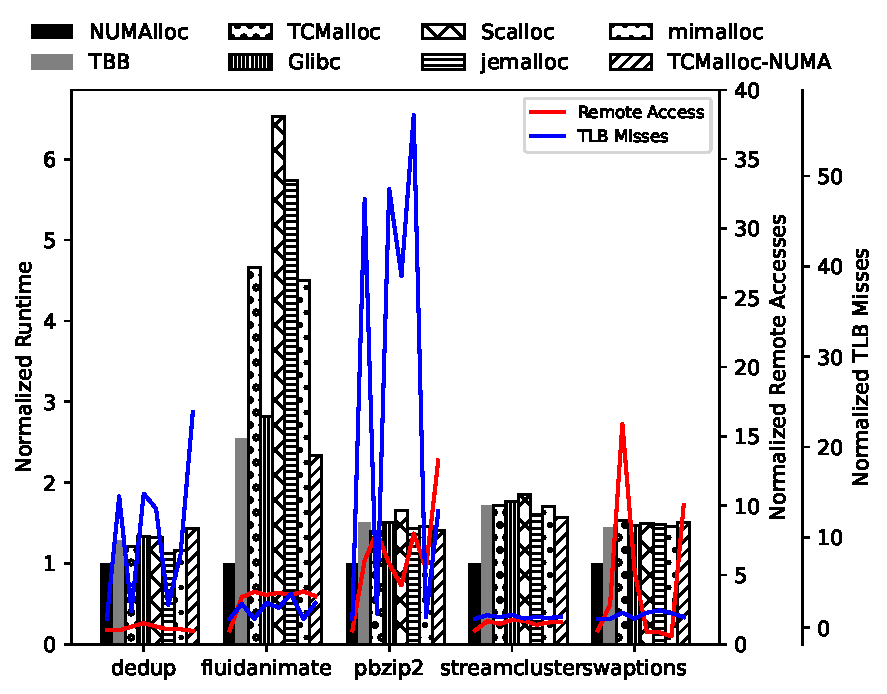
\includegraphics[width=3.5in]{figure/remote-access.pdf}
    \caption{Normalized runtime and the number of remote accesses of different allocators, where all of them are normalized to \NM{}. }
    \label{fig:remoteAccess}
\end{figure}
%\todo{Change "Performance" to runtime, also change the the performance/remote accesses" scale to 8, maybe put NUMAlloc to the first, change TcMalloc to TCMalloc. }

\begin{comment}
\begin{table}[htp]
    \centering
    \footnotesize
    \begin{tabular}{l|c| c|c|c|c|c|c|c|c}
    \multicolumn{2}{c|}{Application} & glibc & \NM{} & TCM & TCM-NUMA & jemalloc & TBB & Scalloc & mimalloc \\ \hline
    \multirow{2}{*}{canneal} & Remote & 772 & 613 & 718   & 626 & 690 & 752 & 655 & 709\\ \cline{2-10}
    & TLB Misses &  & 975  &    &  &1876  & 1910 & 1836 & 1876 \\ \hline
    \multirow{2}{*}{dedup}  & Remote & 35.7 & 23.8 & 23.2 & 32.6 & & 29.9 & 28.4 & 23.7\\ \cline{2-10}
     & TLB &  & 21.6 &    &  & & 31.1 & 42.0  & 19.2\\ \hline
    \multirow{2}{*}{fluidanimate} & Remote  & 784 & 145 & 755 & 902 & & 741 & 798 & 749\\ \cline{2-10}
    5.2
   & TLB  &  & 11.9  &    &  & & 116 & 137 & 100\\ \hline
    \multirow{2}{*}{streamcluster} & Remote  & 762 & 571 & 602 & 548 & & 768 & 497 & 570\\ \cline{2-10}
    &  TLB  &  & 12.1 &    &  & & 1455 & 1410 &  1432\\ \hline
    \multirow{2}{*}{pbzip2} & Remote  &  59.3 & 15.2 & 102 & 98.8 & & 62.5 & 45.8 & 60.4\\ \cline{2-10}
    & TLB &  & 0.8 &    &  & & 98.1 & 66.8 & 26.7 \\ \hline
    \end{tabular}
    \caption{TLB misses when using different allocators. The data shown is mega. }
    \label{tab:characteristics}
\end{table}

\end{comment}

%Table~\ref{tab:characteristics} shows that \NM{} significantly reduces the number of remote accesses and TLB misses due to its region-based design. 

%\todo{Hanmei: maybe we need to get the data on these applications. perf stat -e node-loads, node-load-misses, node-stores, node-store-misses ./APP a.out}



%We  can see that the average value of \NM{} is 0.97 in Machine A and 0.92 in Machine B and it is always the best among all other allocators. The reason that \NM{} got better performance in Machine B is that there are more nodes and more cores in Machine B, which means \NM{} could be very helpful to better to take use hardware resource of multi nodes and cores. but we could get amazing improvement if we shutdown interleaved heap in \NM{} and we will give the data in following sections.In the figure ~\ref{8node-parsec-perf}, we could see more exciting improvement from \NM{}, with average normalized value of 0.92 that is not only the best but also far aware better than all the rest allocators that TCMalloc and jemalloc got 0.99, TCMalloc-NUMA and TBB got roughly 1.07 and 1.01 separately. And also, we can see that the performance of \NM{} is the best for almost each single applications, especially it got 0.17 in fluidanimate and 0.66 in streamcluster which is far better than any of other allocators. As the same thing, the performance of ratrace and canneal is not good here, we will talk about it later after we shut down the interleaved heap.


%In the figure ~\ref{hoard-perf}, we show the normalized performance for Hoard benchmarks in Machine A and Machine B separately. We can see from figure ~\ref{hoard-perf} that the average value of \NM{} is also the best, which is 0.47 that means 2 times faster than default Linux Allocator, and jemalloc got 0.7 and Scalloc got 0.9. In the threadtest, the normalized value of \NM{} is 0.19 , far better than any of others, which means there are few central free list competitions, mainly contributed by properly node management and low overheads operations. For false sharing, \NM{}'s performance is also almost the best as same as Scalloc and jemalloc, which means they could handle false sharing issues very properly. In the larson, \NM{} and TCMalloc are the best, which mainly contributed by their low overheads for allocation and remote de-allocation, but due to our better node management, \NM{} could be better in the Machine B which will be mentioned later. In the figure ~\ref{hoard-perf}, we can also see that \NM{} got lowest average normalized value:0.33, significantly smaller than any of others that TBB got 0.99, Scalloc and jemalloc got roughly 1.14. And also, \NM{} and Scalloc could handle false sharing issue very well, and \NM{} could extremely well reduce central free list competition in threadtest. In larson, \NM{} is the best due to its properly multi-node management. 


\subsection{Memory Consumption}
\label{sec:memory}

%\renewcommand{\arraystretch}{1.5}
\begin{table}[tp]
\footnotesize
	\setlength{\tabcolsep}{0.3em}
  \centering
    \begin{tabular}{|l|r|r|r|r|r|r|r|}
    \hline
    \multirow{2}{*}{Apps}&
    \multicolumn{7}{c|}{Memory Usage (MB)}\\
    \cline{2-8}
    &Linux&\NM{}&TcM&TcM-N&jem&TBB&Scalloc \\ \hline
    \hline
    blackscholes&615&509&621&623&633&615&630\\ \hline
    bodytrack&37&161&45&46&570&37&1994\\ \hline
    canneal&888&879&774&757&1294&888&36149\\ \hline
    dedup&912&1236&983&1023&1389&912&8556\\ \hline
    facesim&560&500&603&601&1133&547&3056\\ \hline
    ferret&184&493&195&183&596&184&3377\\ \hline
    fluidanimate&470&392&483&484&481&470&3437\\ \hline
    raytrace&1288&1472&1092&1543&1287&1288&4398\\ \hline
    streamcluster&113&105&123&121&127&113&193\\ \hline
    swaptions&33&268&16&21&540&37&1817\\ \hline
    vips&228&536&248&269&778&227&3681\\ \hline
    x264&2859&2721&3047&3064&3719&2859&5402\\ \hline \hline  
    Aget&8&74&11&10&93&8&80 \\ \hline
    Apache&8&34&10&9&10&4&42\\ \hline
    Memcached&16&80&25&24&41&18&263\\ \hline
    Mysql&277&732&314&315&500&276& N/A \\ \hline
    Pbzip2&463&747&817&813&1121&454&4881 \\ \hline
    Pfscan&522&542&528&528&535&522&554\\ \hline
    Sqlite3&45&284&60&75&139&44&681 \\ \hline
    \hline
    Total&{\bf 9527}&{\bf 11763}&{\bf 9993}&{\bf 10510}&{\bf 14986}&{\bf 9502}&{\bf 79190}\cr\hline
    \end{tabular}
  \caption{Memory consumption of different allocators. Here, TcM stands for TcMalloc, TcM-N is TcMalloc-NUMA, and jem is jemalloc. \label{tab:memory_consumption}}
\end{table}


We also measure the maximum memory consumption of these allocators.
%For non-server applications, such as \texttt{Aget}, \texttt{Pbscanf}, \texttt{Pbzip2} and all PARSEC applications, we utilized the sum of the \texttt{maxresident} output from the \texttt{time} utility and the size of huge pages, since the \texttt{time }output does not include huge pages. 
%To determine the size of huge pages, a script is used to periodically collect the number of huge pages by reading from \texttt{/proc/meminfo} file, and then the maximum value of huge pages is used. \todo{removed. This is for mmap's huge page, THP usage is counted}
%For server applications, such as \texttt{MySQL}, \texttt{SQLite}, and \texttt{Memcached}, \texttt{Apache}, the maximum memory is collected by the sum of both \texttt{VmHWM} and \texttt{HugetlbPages} fields from \texttt{/proc/PID/status} file, after the corresponding client exits. 
%We always reboot server applications for each single test. 
Memory overhead is listed in Table~\ref{tab:memory_consumption}. Overall, the Glibc allocator has the smallest memory consumption, and TBB is the second-best one. \NM{}'s memory consumption is around \todo{11\%} more than that of the default Linux allocator, but it is better than jemalloc and mimalloc, and is far better than scalloc. 
%Scalloc is the worst one in terms of memory consumption, which consumes around  $8.3\times$ more memory that that of TBB.  

\NM{}'s more memory consumption is mainly due to the following reasons. It allocates a large memory block from the OS. When transparent huge page support is enabled, then all memory will be allocated from huge pages. The same reason also applies to Scalloc, which also allocates a continuous huge region of virtual memory from the underlying OS initially. Comparing to Scalloc, \NM{} makes all threads share the same bag for each size class, as described in Section~\ref{sec:others}, which effectively reduces its memory consumption by multiple times. In total, Scalloc utilizes $7\times$ more memory when transparent huge page support is enabled.  

We further confirmed the memory consumption when transparent huge page support is disabled, which can be seen in Table~\ref{tab:memory_consumption}. The total memory consumption is decreased from \todo{14762} MB to \todo{13128} MB, when transparent huge pages are disabled. In this case, \NM{}'s total memory overhead is comparable to the default Linux allocator. Other allocators will not be affected much by transparent huge pages, since they typically obtain a small chunk from the OS each time, less than the size of a huge page (2MB), then the OS will not allocate physical pages from huge pages by default. \todo{I doubt it} Therefore, we believe that \NM{}'s memory consumption is acceptable. 

%Second, \NM{} may not return the memory to the OS immediately for large pages. However, we believe that its memory consumption is acceptable. 
  %which actually shows the worst case for \NM{}. The OS will utilize huge pages if a memory area is larger than the size of a huge page (2MB). Since \NM{} utilizes \texttt{mmap} to allocate a huge chunk of virtual memory, this makes all heap memory for real objects will be allocated from huge pages. Currently, \NM{} also utilizes 1MB as the superblock for each size class, making objects of a size class that will occupy at least 1MB even if it only uses an object inside. 
 % Therefore, an application with many size classes will waste more memory. \NM{} makes all threads share the same bag for each size class, as described in Section~\ref{sec: others}, which effectively reduces its memory consumption by multiple times. 
 
 %Scalloc has excessive memory consumption, since its design does not support transparent huge pages very well. Similar to \NM{}, Scalloc utilizes a \texttt{mmap} system call to allocate a continuous huge region of virtual memory from the underlying OS. Since every thread will get a virtual span (2MB) for each size class in Scalloc, it will utilize 2MB physical memory even if only a word is touched. Differently, \NM{} avoids this issue as described in Section~\ref{sec: others}.
% the OS will assign a huge page when transparent huge page is enabled by default. Thus, if only one object is allocated from a size class, 
 
\begin{comment}


In Figure~\ref{2node-hoard-mem}, the average normalized value of \NM{} is larger than others, but actually not too much, which is 2.3 for \NM{}, 1.9 for TCMalloc-NUMA and 1.8 for TCMalloc. It is because that proper node management is utilized in \NM{} and also in TCMalloc-NUMA, so that each node also preserves some memory not only thread locals. But we believe that these little more memory overheads are totally acceptable. It is also the same thing for Figure 10, that the average value for \NM{} is a little higher than others, which is 5.3. But in this 8 nodes machine, \NM{} is not the worst, that Scalloc's average value is 25 and jemalloc is 9.4. One main reason that the value of \NM{} is smaller is that we use mini-size bags in \NM{} which is less than the size of one page for small objects and also memories for small objects are shared per node but per cores in Scalloc.
	
\end{comment}


\subsection{Scalability}
\label{sec:scale}

%We also evaluated the scalability of different allocators. 

To validate the scalability of \NM{}, we use four synthetic applications from Hoard~\cite{Hoard}, including \texttt{threadtest}, \texttt{larson}~\cite{Larson}, \texttt{cache-scratch} and \texttt{cache-slash}, which is also employed by existing work~\cite{Scalloc}. We do not use the same applications in Section~\ref{sec:evaluation}, as they are not scalable by design.
%We have verified blacksholes, bodytrack, canneal, and raytrace.
For instance, raytrace has no performance difference when running with 16 threads or 40 threads.
%Therefore, we are using four synthetic applications from Hoard~\cite{Hoard}, including \texttt{threadtest}, \texttt{larson}~\cite{Larson}, \texttt{cache-scratch} and \texttt{cache-slash}, which is also employed by existing work~\cite{Scalloc}. \texttt{larson} simulates a multithreaded server that could respond to requests from different clients, and \texttt{threadtest} is an application that performs a large number of allocations and deallocations within a specified number of threads. Both \texttt{cache-scratch} and \texttt{cache-thrash} test false sharing issues that can be introduced by allocators, where multiple threads are getting and accessing different objects in the same cache line.  
%Passive false sharing is introduced upon deallocations, where a freed object can be utilized by another thread. In contrast, active false sharing is introduced during the initial allocations, where multiple continuous objects sharing the same cache line are allocated to different threads. The synthetic applications have a better scalability by design than other evaluated applications in the last section. 
%Since other allocators cannot specify the configuration, we only evaluate the scalability with different number of threads. 
In the evaluation, we maximize the number of threads on each node for \NM{}. For instance, 32 threads will use 2 nodes, as each node has 16 cores. For other allocators, we only specify the number of threads, and it is up to the OS to determine the scheduling. 
%The corresponding data is shown in Fig.\ref{sythentic-scalability}. All data are normalized to the data of one thread of the Linux's default allocator, where the higher is better.

\begin{figure*}[!th]
    \centering
    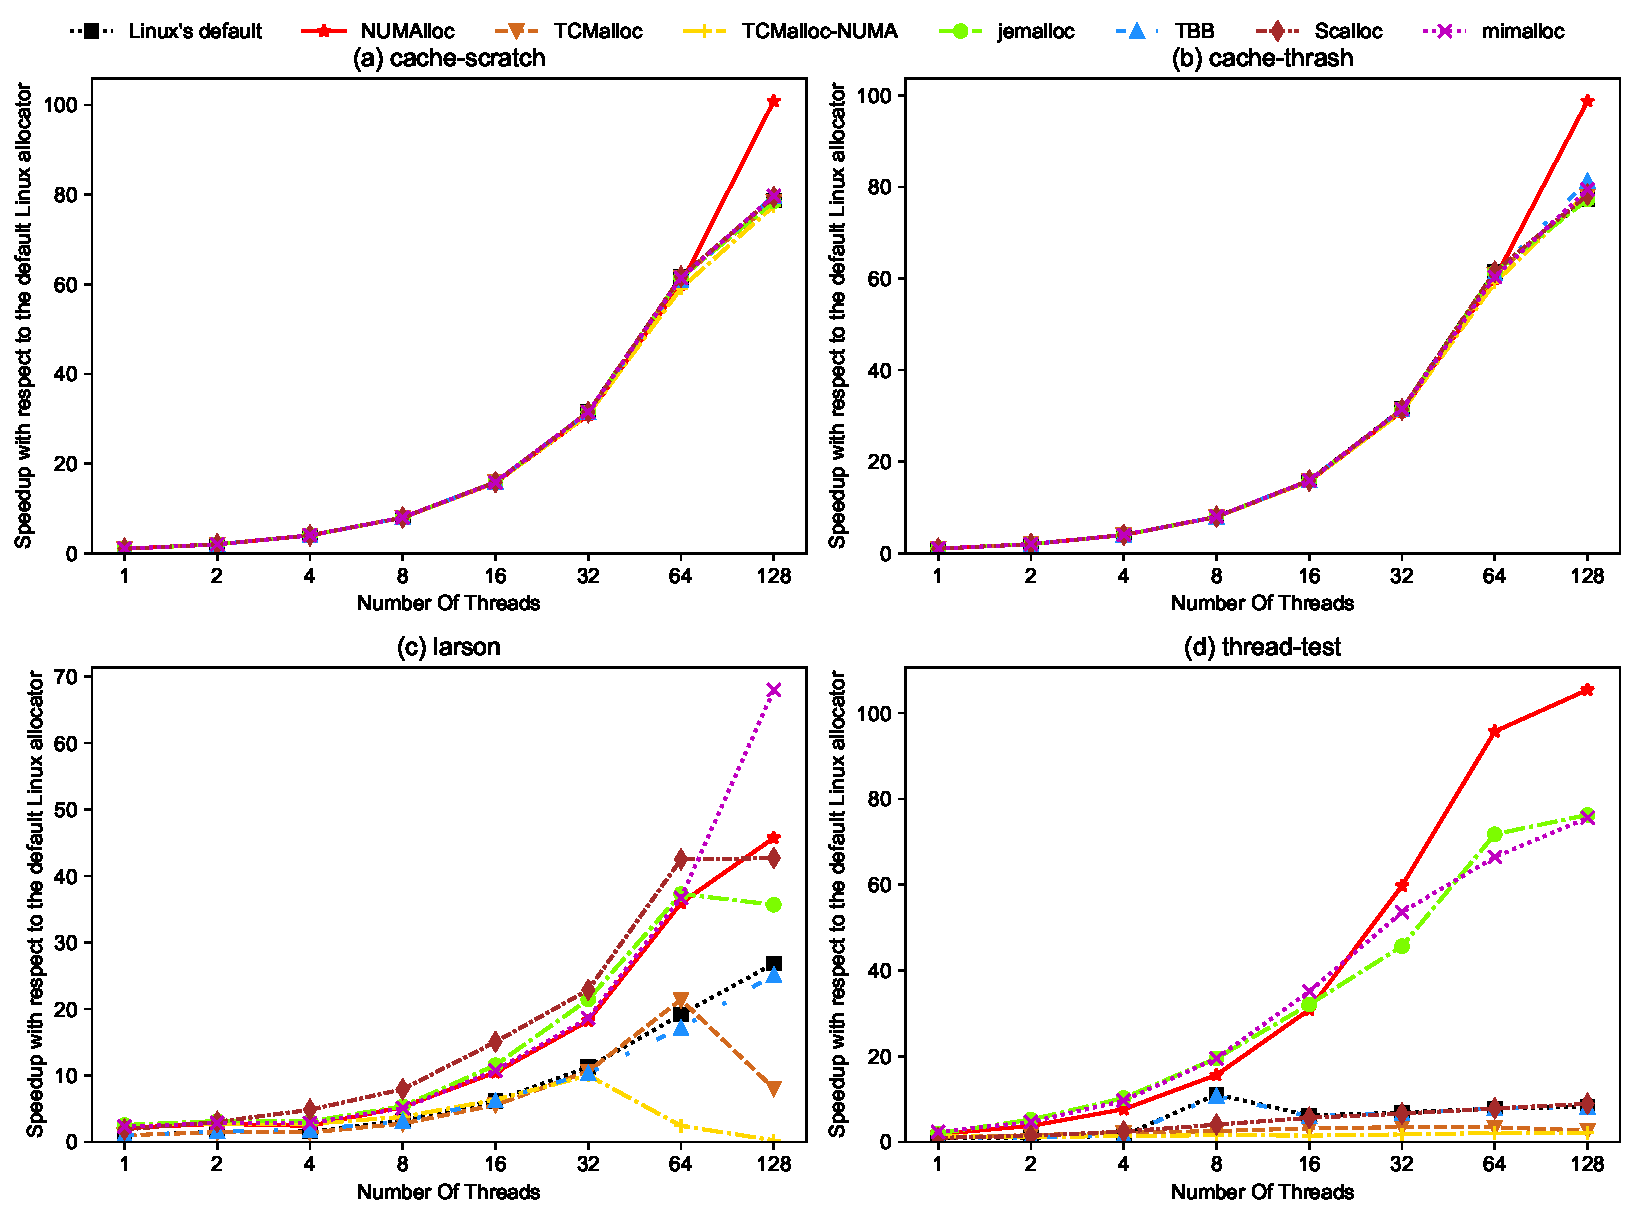
\includegraphics[width=\textwidth]{figure/sythentic-scalobility-new.pdf}
    \caption{Scalability evaluation of different allocators.\\ All data is normalized to the runtime of the default Linux allocator with one thread.}
    \label{sythentic-scalability}
\end{figure*}

Fig.\ref{sythentic-scalability} illustrates different allocators' performance speedup with the increasing number of threads. All data is normalized to the runtime of Linux's default allocator under one thread. Overall, \NM{} has the best performance when the number of threads is 128. Its average speedup is $88\times$, compared to Linux's allocator with one thread, while the second-best allocator -- \texttt{mimalloc} -- has $75\times$ speedup. In contrast, the default Linux allocator only has the speedup of $49\times$. That is, \NM{} has the best scalability.
%When computing the speedup using the data of one thread of each allocator, \NM{}'s average speedup is $65\times$, while the second-best one is $54\times$. 
\NM{} only performs worse than mimalloc for larson with 128 threads, but it performs better for other applications. All of these data indicate that \NM{} is scalable to 128 cores. 
%We don't know the exact reason for this.

\todo{Previous we have analysis of TCMalloc on two cache applications, but I think it's not representative as larson and thread-test}

%Among these applications, \texttt{cache-scratch} tests passive false sharing, and \texttt{cache-thrash} tests active false sharing. False sharing occurs when multiple threads are concurrently accessing different words in the same cache line. 
%Passive false sharing is introduced upon deallocations, where a freed object can be utilized by another thread. In contrast, active false sharing is introduced during the initial allocations, where multiple continuous objects sharing the same cache line are allocated to different threads. 
%For these false sharing tests, we use 100,000 inner-loop, and 100,000 iterations with 8-byte objects.

\begin{comment}
Among these applications, \texttt{cache-scratch} tests passive false sharing, and \texttt{cache-thrash} tests active false sharing. TCMalloc has serious issues of both active and passive false sharing issues, which is the major reason that it does not perform well on both applications. 
\NM{} will not introduce active false sharing, since each thread will get a page of objects initially. Although \NM{} might introduce passive false sharing due to its per-thread cache design, it avoids remote allocations across the node. 
%We believe that is the major reason for its better performance. Other allocators do not have such mechanisms. That is the reason why 
\NM{} is one of the best allocators for \texttt{cache-scratch}, and achieves much better speedup than all other allocators in \texttt{cache-thrash} (30\% faster than the second-best one), as shown in Figure~\ref{sythentic-scalability}. 
\end{comment} 
 %\texttt{larson} is to simulate a multithreaded server that could respond to requests from different clients. \NM{} is around 16\% faster than the second-best allocator--TCMalloc.   \texttt{threadtest} is an application that performs a large number of allocations and deallocations within a specified number of threads. \NM{} is $2.6\times$ faster than the second-best one (jemalloc), when there are 128 threads.
 %Each thread will receive a random number of objects in the beginning, perform a random number of allocation and deallocations to simulate the handler for processing requests, and then pass objects to the next thread. We test \texttt{larson} for 10 seconds with 1,000 objects for 10,000 iterations, where each allocation is between 7 bytes and 2048 bytes. 
 %As shown in Fig.~\ref{sythentic-scalability},  



%Also, it allows to specify how much work to be done between each allocation and deallocation. For \texttt{threadtest}, we use 100 iterations, 1,280,000 allocations, 0 work, and 64-byte objects (for the allocation).  This benchmark will stressfully test the performance overhead of allocation and deallocation. For this application, 
 %since every thread will has its own heap and it only imposes some when getting objects from the shared bag. But \NM{} obtains a number of objects at a time, at the page level, which significant reduce the possibility of contention. 


%On average,  \NM{} is running 79\% faster than the second-best one (Scalloc), and $2.2\times$ faster than the default Linux allocator. Multiple reasons contribute to the good performance of \NM{}: \NM{} imposes very minimal system call overhead, and little synchronization overhead. Also, it introduces less remote accesses than all other allocators, due to its NUMA-aware design. Other allocators have more or less false sharing issue, or incurs remote accesses.  
%\todo{Surprisingly, TCMalloc and  }.



%That is the reason why it has a good performance as the Linux allocator for \texttt{cache-thrash}.

 
\begin{comment}

\begin{figure}[!ht]
    \centering
    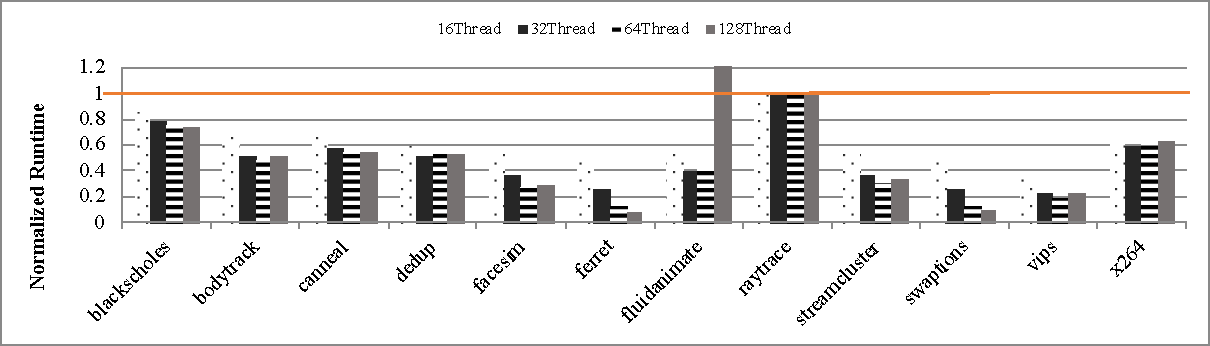
\includegraphics[width=5.5in]{figure/scalobility-pthread.pdf}
    \caption{Normalized performance of Linux's default allocator without binding for PARSEC benchmarks in Machine B}
    \label{pthread-scalibity}
\end{figure}
We will evaluate the scalability on 8threads, 16threads, 32 threads, 64 threads and 128 threads. 
(one node, two node, four nodes, and 8 nodes). 
	
\end{comment}


\subsection{Design Choices}
\label{sec:design}

This section further confirms \NM{}'s multiple design choices, and all results shown in this section are normalized to the data of the default Linux allocator.  

%Based on our analysis, there are two reasons for this performance speedup. First, a thread will not be migrated to a different core, avoiding unnecessary remote accesses caused by cross-node migration, as further discussed in Section~\ref{sec:intro}. Second, \NM{}'s thread binding balances the workload, thus reducing the congestion of interconnect or one memory controller.
\subsubsection{Choices of Thread Binding}
\label{sec: threadbinding}

% \begin{figure*}[!h]
%     \centering
%     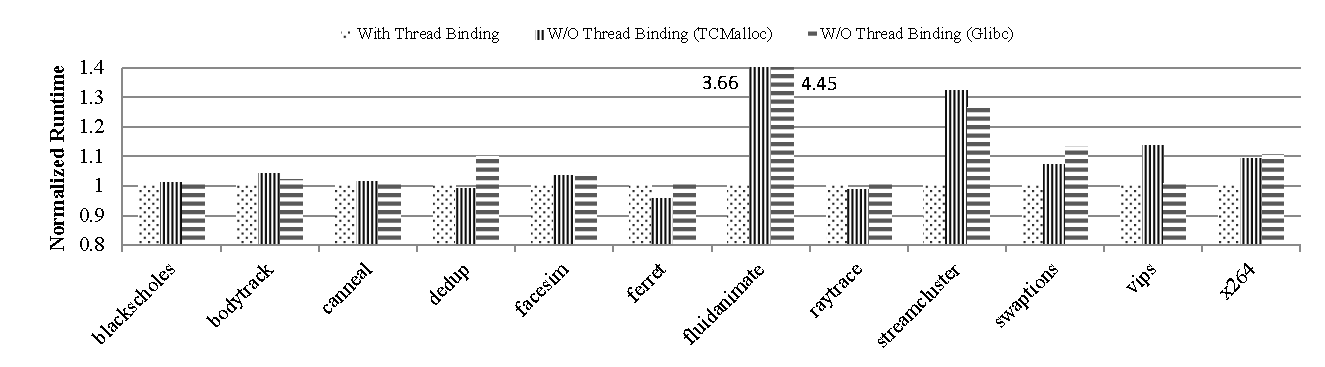
\includegraphics[width=6in]{figure/WO-pthread-binding3.pdf}
%     \caption{Normalized runtime with and without node-balanced thread binding for Glibc and TCMalloc.} 
%     \label{binding-pthread-scalibity}
% \end{figure*}

% \begin{figure*}[!ht]
%     \centering
%     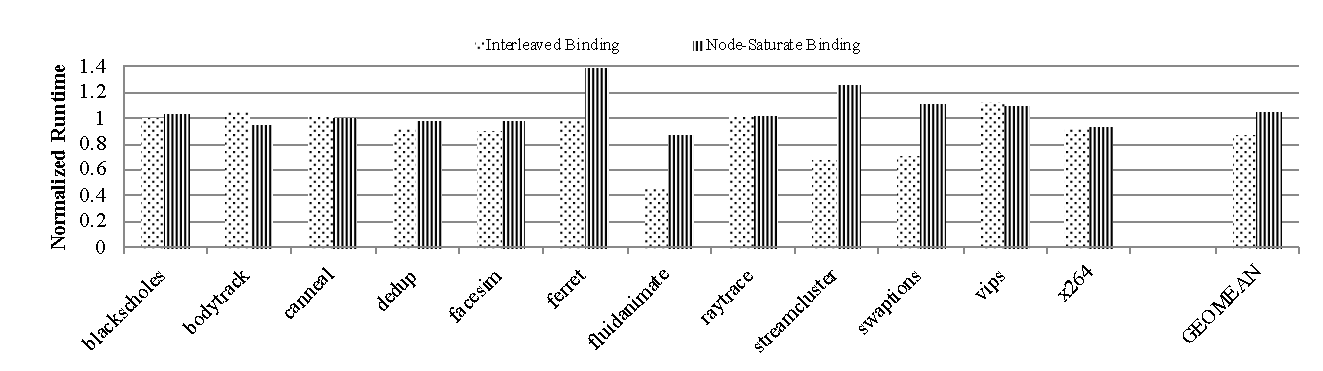
\includegraphics[width=5.5in]{figure/binding-policy.pdf}
%     \caption{ Node-Interleaved vs. Node-Saturate binding for Glibc, where results are normalized to those without binding.}
%     \label{fig:binding-policy}  
% \end{figure*}

\begin{figure*}[!h]
\centering
\subfloat[Normalized runtime with and without node-balanced thread binding for Glibc and TCMalloc.]{
  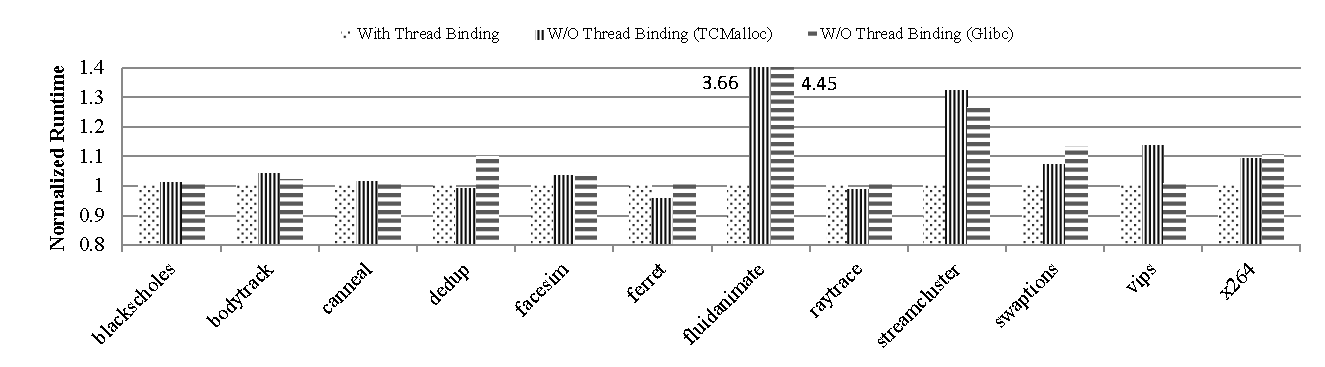
\includegraphics[width=5.5in]{figure/WO-pthread-binding3.pdf}
}

\subfloat[Normalized runtime with node-interleaved binding and node-saturate binding for Glibc.]{
  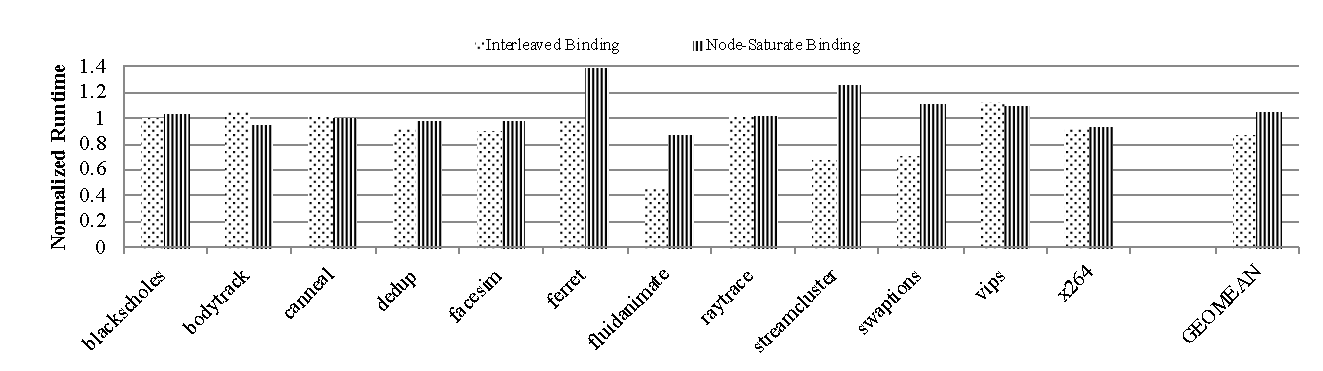
\includegraphics[width=5.5in]{figure/binding-policy.pdf}
}
\caption{Performance results with the impact of Thread Binding.}
\label{binding-pthread-scalibity}
\end{figure*}

Fig.\ref{binding-pthread-scalibity}(a) shows the performance difference with and without thread binding for two allocators, Glibc and TCMalloc. Here node-balanced binding strategy is adopted. We do not evaluate \NM{} directly, since its mechanism is tightened to thread binding, such as its origin-based memory management, metadata allocation. We observe that the thread binding improves the performance significantly for some applications. As shown in Fig.\ref{binding-pthread-scalibity}(a), with the thread binding, \texttt{fluidanimate} runs around $4.45\times$ faster on Glibc and $3.66\times$ faster on TCMalloc. \texttt{streamcluster} runs more than 20\% and 30\% faster than the one without the binding. This clearly indicates that the thread binding will benefit the performance overall, which should be included in the memory allocator by default. 

% In particular, threads are bound to different nodes in a round-bin way, called node-balanced binding, which is the same as \NM{}.

We further compare the node-interleaved thread binding with node-saturate thread binding. For node-saturate binding, we bind the maximum possible number of threads (same as the number of cores) to a node and then switch to the next node. As shown in Fig.\ref{binding-pthread-scalibity}(b), the node-interleaved thread binding is almost always better than node-saturate thread binding, except for \texttt{bodytrack}. On average, node-interleaved binding is around 19\% faster than node-saturate one. This indicates that people should use node-interleaved binding, if they would like to employ all hardware cores. However, if they only want to use partial cores to run one application, then node-saturate binding could be a better choice. \NM{} allows users to adjust the binding option.  

% , proving the effectiveness of Node-Balanced thread binding.

\subsubsection{Interleaved Heap} 
\label{sec:interleavedheap}

\begin{figure*}[!ht]
    \centering
    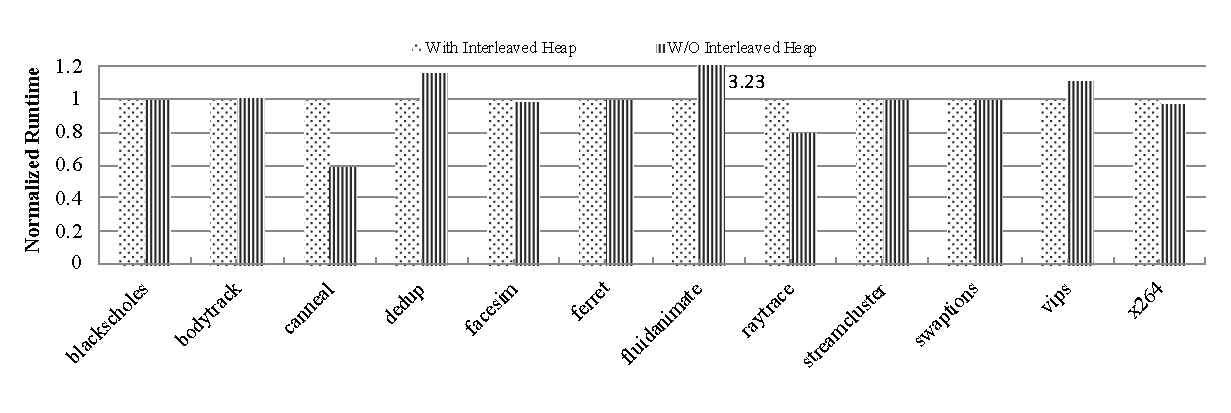
\includegraphics[width=5.5in]{figure/interleavedheap.pdf}
    \caption{Normalized runtime with and without the interleaved heap for \NM{}.  \label{fig:interleavedheap}}
\end{figure*}

We also evaluate the potential benefit of the interleaved heap. The performance data is shown in Fig.\ref{fig:interleavedheap}. 
% Note that we have evaluated all PARSEC applications listed in Section~\ref{sec:performance}.
Based on the figure, we have the following conclusion: the interleaved heap will benefit (or at least has no harmful impact on) the performance for most applications. Some applications, such as \texttt{fluidanimate}, will have the performance speedup of $3.23\times$ with the interleaved heap. However, applications having a large portion of time spent in the serial phase, such as \texttt{canneal} and \texttt{raytrace}, may not have good performance with the interleaved heap support. 
We investigated the underlying reason for this. With the interleaved heap, \NM{} allocates the memory from all nodes in an interleaved way, instead of from the local node (based on the default first-touch policy). Therefore, some private objects that are allocated in a remote node may introduce unnecessary overhead due to remote access. Further, upon each allocation, \NM{}  checks the callstack to confirm whether an allocation is from a potentially shared heap, which also introduces some overhead. Therefore, the interleaved heap will be enabled by default, unless programmers know that it will not benefit the performance.

A simple metric is to use the portion of the serial phase inside multithreaded applications.  Programmers may turn off the interleaved heap for applications that are mostly running in serial phases. That is, the interleaved heap will harm the serial execution, but may benefit the parallel execution because of its load balance. It is easy to turn on/off the interleaved heap via a compilation flag or the environment variable.  

\todo{other design choices: THP's impact on performance, origin-based deallocation, autonuma's impact...}

%, except applications with a large portion of serial phase (e.g., \texttt{canneal} and \texttt{raytrace})

%The interleaved heap could be utilized to avoid load imbalance issue for shared objets. 

%However, there are two issues for the interleaved heap. First, the allocator may not know whether an object is shared or not at the first time. Therefore, all objects that are allocated in the main heap (before creating any child thread) will be treated as the shared heap. Second, some applications are spending too much time in the serial phase, where the interleaved heap cannot benefit the performance for the serial phase. 





%figure ~\ref{parsec-no-interleaved-perf} we show some performance results of some applications that got significant different values after we shut down interleaved heap for \NM{}. We can see that for some applicatios with less data sharing between threads like ratrace and canneal, \NM{} could got significant improvements due to its low overheads and proper memory management. But for some other applications with intensive memory operations and sharing like fluidanimate, shutting down interleaved heap could hurt performance, since interleaved heap could help to distributed resource contention evenly over multi-nodes and then got low overheads.

%\subsubsection{Selective Huge Pages} 
%\label{sec:hugepage}

%Since the machine utilizes transparent huge pages by default, we evaluate the performance impact of huge page support on another machine with 2 NUMA-node, without enabling the transparent huge pages.
% A, the 2-node machine. We only utilize PARSEC applications for this evaluation. 

%\begin{figure}[!h]
%    \centering
%    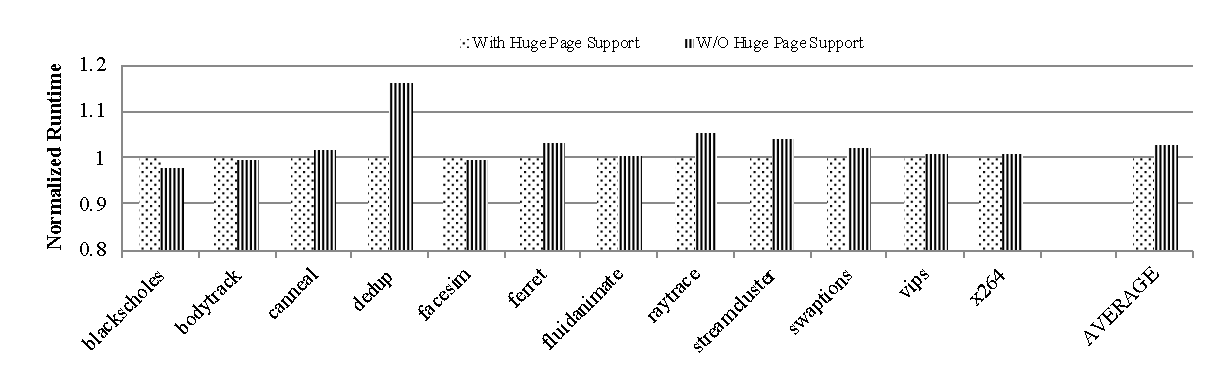
\includegraphics[width=3.2in]{figure/hugepage.pdf}
%    \caption{Normalized runtime with and without selective huge pages.}
%    \label{fig:hugepage}
%\end{figure}

%The results are shown in Figure~\ref{fig:hugepage}. When integrating with selective huge pages, \NM{} achieves a significantly better performance for \texttt{dedup}, where the performance difference is around 15\%. On average, the selective huge pages improves the performance of all evaluated applications about 2.5\%, and will not hurt the performance. This clearly indicates that it is beneficial to have selective huge pages for the NUMA architecture, especially given the fact of increasing memory size of hardware trend.  


